% Created 2020-09-17 qui 18:18
% Intended LaTeX compiler: pdflatex
\documentclass[11pt]{article}
\usepackage[utf8]{inputenc}
\usepackage{lmodern}
\usepackage[T1]{fontenc}
\usepackage[top=3cm, bottom=2cm, left=3cm, right=2cm]{geometry}
\usepackage{graphicx}
\usepackage{longtable}
\usepackage{float}
\usepackage{wrapfig}
\usepackage{rotating}
\usepackage[normalem]{ulem}
\usepackage{amsmath}
\usepackage{textcomp}
\usepackage{marvosym}
\usepackage{wasysym}
\usepackage{amssymb}
\usepackage{amsmath}
\usepackage[theorems, skins]{tcolorbox}
\usepackage[style=abnt,noslsn,extrayear,uniquename=init,giveninits,justify,sccite,
scbib,repeattitles,doi=false,isbn=false,url=false,maxcitenames=2,
natbib=true,backend=biber]{biblatex}
\usepackage{url}
\usepackage[cache=false]{minted}
\usepackage[linktocpage,pdfstartview=FitH,colorlinks,
linkcolor=blue,anchorcolor=blue,
citecolor=blue,filecolor=blue,menucolor=blue,urlcolor=blue]{hyperref}
\usepackage{attachfile}
\usepackage{setspace}
\usepackage{tikz}
\usepackage[american, english]{babel}
\usepackage{minted}
\author{Gabriel Petrini}
\date{September 10th, 2020}
\title{GEV}
\begin{document}

\maketitle
\tableofcontents

\begin{minted}[frame=lines,fontsize=\scriptsize,linenos]{elisp}
(require 'org-attach-screenshot)
\end{minted}

\section{Pre-class reading: \href{http://eml.berkeley.edu/books/choice2nd/Ch04\_p76-96.pdf}{Train (2009, Ch 4.1--4.2)}}
\label{sec:org1985b58}

\subsection{Reading Quiz}
\label{sec:org2fff647}
\begin{enumerate}
\item Explain why mixed logit is such a popular model, according to Train. What are its strong points vis-à-vis the IIA problem?
\item What are the computational drawbacks to mixed logit?
\item What are two names for a mixed logit model that has a discrete mixing distribution?
\item Explain why the EM algorithm is a potentially powerful tool for estimating discrete choice models.
\item How does the EM algorithm work? Why does it work?
\end{enumerate}


\section{Review}
\label{sec:orgb6d108f}

\subsection{Red bus / blue bus choice set}
\label{sec:orgb61cfa8}

\begin{itemize}
\item As we discussed last time, adding another bus results in odd substitution patterns
\item This is because of the IIA property of multinomial logit models
\end{itemize}

\begin{center}
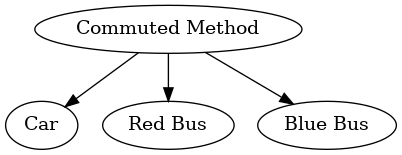
\includegraphics[width=.9\linewidth]{unnested.png}
\end{center}


\subsection{Nesting the choice set}
\label{sec:orgdb56363}
One way to get around IIA is to \textbf{nest} the choice set
\begin{itemize}
\item Nesting explicitly introduces correlation across alternatives within the same nest
\end{itemize}


\begin{center}
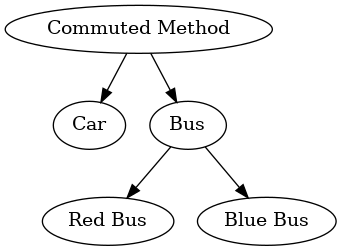
\includegraphics[width=.9\linewidth]{nested.png}
\end{center}


\subsection{Other cases where nesting is useful}
\label{sec:orgab23ed6}

\textbf{Elections}

\begin{itemize}
\item Suppose we have two candidates, A and B
\item If we introduce C, whose platform resembles B, what will new vote shares be?
\item (Primary elections are a kind of nesting)
\end{itemize}

\textbf{Product markets}
\begin{itemize}
\item Nesting ``branded'' and ``generic'' products (e.g. branded vs. micro-brewed beer)
\item But some consumers won't purchase either type of the product
\item Ignoring non-buyers, will give misleading price elasticities of demand
\end{itemize}

\section{Nested Logit}
\label{sec:orgff15ae3}

Coming back to the red bus/blue bus problem, we would like some way for the errors for the red bus to be correlated with the errors for the blue bus
\begin{itemize}
\item The \textbf{nested logit} allows a nest-specific error:
\end{itemize}

\begin{align*}
U_{i,RedBus}&=u_{i,RedBus\phantom{e}}+\nu_{i,Bus}+\lambda\epsilon_{i,RedBus}\\
U_{i,BlueBus}&=u_{i,BlueBus}+\nu_{i,Bus}+\lambda\epsilon_{i,BlueBus}\\
U_{i,Car}&=u_{i,Car\phantom{eBus}}+\nu_{i,Car}+\lambda\epsilon_{i,Car}
\end{align*}

where:

\begin{enumerate}
\item \(\nu_{ik}+\lambda\epsilon_{ij}\) is distributed Type I Extreme Value
\item The \(\nu\)'s and the \(\epsilon\)'s are independent
\item \(\epsilon_{ij}\) is distributed Type I extreme value
\item Distribution of \(\nu_k\)'s is derived in Theorem 2.1 of \textcite{cardell1997}
\end{enumerate}

Composite error term for car is independent from either the red bus error or the blue bus error  

\begin{itemize}
\item If we added a yellow bus, all errors in the bus nest would be independent conditional on choosing to take a bus (i.e. \textbf{IIA within nest})
\item But the bus nest errors are correlated from the viewpoint of the top level (i.e. before conditioning on nest choice)
\item Note: adding two extreme value errors does .hi[not] give back an extreme value error
\begin{itemize}
\item But the difference between two T1EV errors is distributed logistic
\end{itemize}
\end{itemize}

More important than the exact error distribution is the choice probabilities:
\begin{align*}
P_{iC}&=\frac{\exp(u_{iC})}{\left[\exp\left(\frac{u_{iRB}}{\lambda}\right)+\exp\left(\frac{u_{iBB}}{\lambda}\right)\right]^{\lambda}+\exp(u_{iC})}\\
P_{iRB}&=\frac{\exp\left(\frac{u_{iRB}}{\lambda}\right)\left[\exp\left(\frac{u_{iRB}}{\lambda}\right)+\exp\left(\frac{u_{iBB}}{\lambda}\right)\right]^{\lambda-1}}{\left[\exp\left(\frac{u_{iRB}}{\lambda}\right)+\exp\left(\frac{u_{iBB}}{\lambda}\right)\right]^{\lambda}+\exp(u_{iC})}
\end{align*}


Not particularly intuitive, but can break it down into parts \(P(B)P(RB|B)\):
\begin{align}
P_{iRB}&=\left(\frac{\left[\exp\left(\frac{u_{iRB}}{\lambda}\right)+\exp\left(\frac{u_{iBB}}{\lambda}\right)\right]^{\lambda}}{\left[\exp\left(\frac{u_{iRB}}{\lambda}\right)+\exp\left(\frac{u_{iBB}}{\lambda}\right)\right]^{\lambda}+\exp(u_{iC})}\right)\times\label{eq:pbus}\\
&\phantom{\times\times}\left(\frac{\exp\left(\frac{u_{iRB}}{\lambda}\right)}{\exp\left(\frac{u_{iRB}}{\lambda}\right)+\exp\left(\frac{u_{iBB}}{\lambda}\right)}\right)\nonumber
\end{align}

\section{Nested Logit Estimation}
\label{sec:org61e2e1c}

The log likelihood can then be written as:
\begin{align*}
\ell&=\sum_{i=1}^N\sum_{j\in J}(d_{ij}=1)\ln(P_{ij})\\
&= \sum_{i=1}^N\left[(d_{iC}=1)\ln(P_{iC})+\sum_{j\in J_B}(d_{ij}=1)\ln(P_{iB}P_{ij|B})\right]\\
&=\sum_{i=1}^N\left[(d_{iC}=1)\ln(P_{iC})+\sum_{j\in J_B}(d_{ij}=1)(\ln(P_{iB})+\ln(P_{ij|B}))\right]\\
&=\sum_{i=1}^N\Bigg[(d_{iC}=1)\ln(P_{iC})+(d_{iBB}=1+d_{iRB}=1)\ln(P_{iB})\\
&\qquad+\left.\sum_{j\in J_B}(d_{ij}=1)\ln(P_{ij|B})\right]
\end{align*}

Could estimate a nested logit by straight maximum likelihood.  An alternative follows from decomposing the nests into the product of two probabilities: \(P(RB|B)P(B)\)

\begin{itemize}
\item In order to do this, however, first decompose \(u_{RB}\) into two parts:
\end{itemize}
\begin{align*}
u_{iRB}&=u_{iB}+u_{iRB|B}
\end{align*}
\begin{itemize}
\item We also need to choose normalizations:

\begin{itemize}
\item \(u_{iC} = 0\)
\item \(u_{iBB|B} = 0\)
\end{itemize}

\item So we will estimate \((\beta_{B},\beta_{RB}, \gamma,\lambda)\) where \(\gamma\) corresponds to the \(Z\)'s (alt-specific)
\end{itemize}

Note that our normalizations imply the following observable components of utility
\begin{align*}
u_{iC}&=0\\
u_{iBB}&=\beta_{B}X_{i}+\gamma (Z_{BB}-Z_{C})\\
u_{iRB}&=(\beta_{B}+\beta_{RB})X_{i}+\gamma (Z_{RB}-Z_{C})
\end{align*}

\begin{itemize}
\item Now estimate \(\beta_{RB}\) and \(\gamma\) in a 1st stage using only observations that chose bus, \(N_B\):
\end{itemize}
\begin{align*}
\ell_1&=\sum_{i=1}^{N_B}(d_{iRB}=1)(u_{iRB|B}/\lambda)+\ln\left(1+\exp(u_{iRB|B}/\lambda)\right)
\end{align*}

\begin{itemize}
\item The \(1\) in the \(\ln()\) operator corresponds to \(\exp(u_{iBB|B}/\lambda)\) since \(u_{iBB|B} = 0\)
\end{itemize}


Now consider the term in the numerator of \(P(B)\) in \eqref{eq:pbus}.  We can rewrite this as:
\begin{align*}
\left[\exp\left(\frac{u_{iRB}}{\lambda}\right)+\exp\left(\frac{u_{iBB}}{\lambda}\right)\right]^{\lambda}&=
\exp(u_{iBB})\left[\exp\left(\frac{u_{iRB|B}}{\lambda}\right)+1\right]^{\lambda}\\
&=\exp(u_{iBB}+\lambda I_{iB})
\end{align*}

where \(I_{iB}\) is called the .hi[inclusive value] and is given by:
\begin{align*}
I_{iB}&=\ln\left(\exp\left(\frac{u_{iRB|B}}{\lambda}\right)+1\right)
\end{align*}

Note: looks like \(E\left(\text{utility}\right)\) associated with a particular nest (minus Euler's constant)


Taking the estimates of \(u_{iRB|B}\) as given and calculating the inclusive value, we now estimate a second logit to get \(\beta_B\):
\begin{align*}
\ell_2&=\sum_i(d_{iB}=1)(u_{iBB}+\lambda I_{iB}-u_{iC})+\ln(1+\exp(u_{iBB}+\lambda I_{iB}-u_{iC}))
\end{align*}

\begin{itemize}
\item Could do all this because log of the probabilities was additively separable. Consider the log likelihood
\end{itemize}
contribution of someone who chose red bus:
\begin{align*}
\ln(P_{iB}(\beta_{B},\beta_{RB},\gamma,\lambda))&+\ln(P_{iRB|B}(\beta_{RB},\gamma))
\end{align*}

\begin{itemize}
\item We get estimates of \(\beta_{RB}\) and \(\gamma\) only from the second part of log likelihood

\item Then we take these as given when estimating \(\beta_{B}\) and \(\lambda\)
\end{itemize}


\section{The Nested Logit as a Dynamic Discrete Choice Model}
\label{sec:org4d4c9fa}

Instead of having individuals know their full error, consider the case where the error is revealed in stages

\begin{itemize}
\item First individuals choose whether or not to ride the bus and there is an extreme value error associated with both the bus and the car option
\item Individuals take into account that if they choose the bus option they will get to make a choice about which bus in the next period (option value)
\item With the errors in the second choice also distributed Type I extreme value, independent from each other, and independent from the errors in the first period, the expectation on the value of the second period decision is \(\lambda I_{iB}\) plus Euler's constant.
\end{itemize}


\subsection{Proposition 1 \cite{mcfadden1978}}
\label{sec:org4183645}
Let \(Y_{j}=e^{u_{j}}\). Suppose we have a function \(G(Y_{1},...,Y_{{J}})\) that maps from \(R^{{J}}\) into \(R^1\)

If \(G\) satisfies:
\begin{enumerate}
\item \(G\geq 0\)
\item \(G\) is homogeneous of some degree \(k\)
\item \(G\rightarrow \infty\) as \(Y_{j}\rightarrow \infty\) for any \(j\)
\item Cross partial derivatives weakly alternate in sign, beginning with \(G_{i}\geq 0\)
\end{enumerate}


then:
\begin{align*}
F(u_1,...,u_\mathcal{J})&=\exp\left[-G(Y_1,....,Y_{J})\right]
\end{align*}
is the cumulative distribution of a multivariate extreme value function and:

\begin{align*}
P_{i}&=\frac{Y_{i}G_{i}}{G}
\end{align*}
where \(G_i\) denotes the derivative of \(G\) with respect to \(Y_i\)

\section{Logit from GEV}
\label{sec:org33f13e0}

Another way of thinking about the last statement is that:
\begin{align*}
P_i&=\frac{\partial \ln(G)}{\partial u_i}
\end{align*}

\begin{itemize}
\item For the multinomial logit case, the \(G\) function is:
\end{itemize}
\begin{align*}
G&=\sum_{j=1}^{{J}}\exp(u_j)
\end{align*}
with the derivative of the log of this giving multinomial logit probabilities

\begin{itemize}
\item But \(\ln(G)\) (plus Euler's constant) is .hi[also] expected utility

\item In fact, for all GEV models \(\ln(G)\) is expected utility!
\end{itemize}

Suppose a nested logit model with two nests \((F,NF)\) and a no-purchase option \(N\)

\begin{itemize}
\item The \(G\) function is then:
\end{itemize}
\begin{align*}
G&=\left(\sum_{j\in F}\exp(u_j/\lambda_F)\right)^{\lambda_F}+\left(\sum_{j\in NF}\exp(u_j/\lambda_{NF})\right)^{\lambda_{NF}}+\exp(u_N)
\end{align*}

\begin{itemize}
\item Differentiating \(\ln(G)\) (the expected utility function) with respect to \(u_j\) where \(k\in F\) yields the probability \(k\) is chosen:
\end{itemize}

\begin{align*}
P_k&=\frac{\exp(u_k/\lambda_F)\left(\sum_{j\in F}\exp(u_j/\lambda_F)\right)^{\lambda_F-1}}{\left(\sum_{j\in F}\exp(u_j/\lambda_F)\right)^{\lambda_F}+\left(\sum_{j\in NF}\exp(u_j/\lambda_{NF})\right)^{\lambda_{NF}}+\exp(u_N)}
\end{align*}

\subsection{Overlapping nests (Bresnahan et al., 1997)}
\label{sec:orgb35c84f}

We can also come up with more general nesting structures

\begin{itemize}
\item \textcite{bst1997} model 4 overlapping nests for computers:

\item Branded but not Frontier \(\{B,NF\}\)
\item Generic but Frontier  \(\{NB,F\}\)
\item Branded and Frontier  \(\{B,F\}\)
\item Generic but not Frontier  \(\{NB,NF\}\)

\item Use the model to understand market power in PC sector in late 1980s

\item Overlapping nests explain coexistence of imitative entry and innovative investment
\end{itemize}


\section*{References}
\label{sec:org568be15}
\end{document}